\chapter{Automatic Speech Recognition}

V této kapitole se čtenář seznámí s některými základními paradigmaty ASR, dozví se, jak ASR proces vypadá. Zároveň je zde představen úvodní formalismus problematiky.

Nejprve se čtenář dočte o tom, co to vlastně ASR je, poté jak ASR probíhá. Nahlédne pod pokličku základů zpracování signálu, inherentních jazykových omezení, modelování ASR systémů a nakonec i hodnocení kvality výstupu.

\section{Co je to ASR}

Moderní ASR využívá teoretický model, založený na pravděpodobnostních vlastnostech akustických pozorování, který formalizuje převod mluveného slova do textu. Přeneseně se takto označují i konkrétní systémy a implementace, které tohoto modelu využívají. 

Ultimátním cílem  je získat systém, který bude v reálném čase převádět přirozenou lidskou řeč na text se stoprocentní úspěšností pro všechna slova, nezávisle na zkreslení vstupních zařízení, okolním ruchu, nebo přízvuku mluvčích. Již v minulosti ASR systémy dosahovaly i kolem devadesátiprocentní úspěšnosti \cite{jelinek_1976}.

\section{Postup rozpoznávání}

\begin{figure}[h]
	\centering
	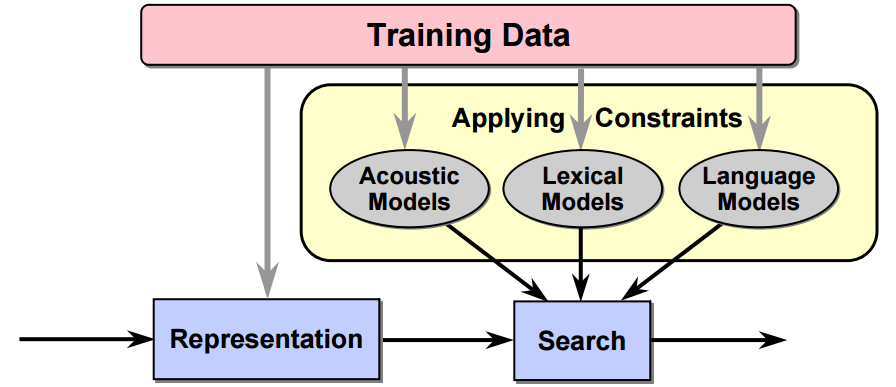
\includegraphics[width=140mm]{img/asr_process.png}
	\caption{Hlavní součásti ASR systému \cite{mit_asr_2003}}
	\label{fig:asr_process}
\end{figure}

Obrázek \ref{fig:asr_process} ukazuje, že samotný návrh systému je poměrně přímočarý.
\\\\*
Zásadními milníky systému jsou:

\begin{itemize}
\item Jak zpracovat signál?
\item Jak se popasovat s omezeními?
\item Jak nalézt optimální výstup?
\end{itemize}

\section{Reprezentace a zpracování signálu}

Pro reprezentaci a zpracování signálu se dříve běžně využívaly dva druhy analýzy -- analýza pomocí {\sl discrete-time} Fourierovy transformace (\nom{DTFT}{Discrete-Time Fourier Transform}) a její důsledek -- Cepstrální analýza (\nom{CA}{Cepstral Analysis}). Dnes se pro tyto účely využívá pro změnu důsledků druhé zmíněné metody v podobě \nom{MFCC}{Mel-frequency cepstral coefficients} (Mel-Frequency Cepstral Coefficients) analýzy.

Všechny tyto metody se snaží zachytit příznaky v signálu, které lze dále využít pro jeho zpracování.

Fourierovská analýza je prvotním způsobem, jak signál zpracovat a reprezentovat. Původně se využívalo vztahu DTFT samotného, posléze již i jeho dalšího zpracování \cite{shaug_2003}.

Je zajímavé, že CA vznikla jako nástroj analýzy časového rozvoje seismických signálů vzniklých zemětřeseními, či explozemi. Měla pomoci nalézt především hloubku generátoru seismických signálů analýzou odezvy těchto signálů \cite{bogert_1963}.

CA využívá předpokladu, že signál je výstup lineárního časově invariantního (\nom{LTI}{Linear Time-Invariant} -- Linear Time-Invariant) systému; tedy že je to konvoluce vstupu a impulsové odezvy. Pokud se chceme zabývat charakterizací tohoto modelu, musíme projít procesem dekonvoluce. A CA je právě postup, využívaný pro takovouto LTI dekonvoluci \cite{tohkura_1987}.

MFCC iteruje na principu CA, především se soustředí na přiblížení principu CA lidskému konceptu vnímání tím, že rozprostírá frekvence na mel stupnici ({\sl mel scale}) \cite{hossan_2010}.

\section{Zdroje omezení mluvené komunikace}

Při předávání informace mluvenou řečí může běžně docházet ke zkreslení řečené informace díky několika nepříjemným faktorům, které mohou (a budou) ASR systému působit nepříjemnosti. Těmto omezením se nelze vyhnout, proto jsou ASR systémy nuceny brát v potaz rozličné nepřesnosti a snažit se tyto eliminovat.

Práci už tak nepříjemnou nezlehčuje ani fakt, že omezení nejsou konstantně daná; lze je pouze taxonomizovat a obcházet.
\\\\*
Patří sem například:

\begin{itemize}
\item Akustická omezení -- lidský hlasový aparát trpí, jako každý jiný komplexní systém, také svými neduhami (vrozené vady aparátu, variabilita ústní klenby, velikost ústního otvoru, ...)
\item Fonetická omezení -- \uv{kolemjdoucí paní} - \uv{kolem jdou cíp a ní}
\item Fonologická omezení -- například splynutí \uv{s} a \uv{š} do jednoho dlouhého fonému - \uv{lezeš shora}
\item Fonotaktická omezení -- kupříkladu zjednodušení konsonantických shluků u menších dětí (\uv{uličnice} - \uv{ulitite}), nebo nesmyslná, rádoby přejatá slova (\uv{sympathetic} - \uv{sympatetický})
\item Syntaktická omezení -- \uv{jedu na výlet do Českých Budějovic} - \uv{Českých výlet na Budějovic jedu do}
\item Sémantická omezení -- \uv{zapal sirku} - \uv{zapal si ruku}
\item Lexikální omezení -- \uv{šuplánek} ani \uv{niplavý} nejsou česká slova a nemají tedy žádnou projekci v našem vědomí
\end{itemize}

a mnohá další.

Často také mluvíme o specifikách mluvčího. Každý je svým způsobem unikátní, jeho hlas je taktéž. Navíc, jedincův hlas se může různit od sebe samého i v důsledku únavy, nemoci, nebo psychického rozpoložení.

Nejčastěji však bojujeme s nepřízní okolí a nepřesností prostředků záznamu zvuku. Výrazný šum na pozadí a špatně zvolené zařízení a technologie záznamu zvuku dokáží nejednomu ASR systému pěkně zavařit.

\section{Modelování systému}

V ASR procesu se stroj pokouší nalézt co možná nejlepší shodu získaného signálu (reprezentace přirozené řeči) a posloupnosti písmen (slov, vět). Abychom něčeho podobného mohli dosáhnout, musíme navrhnout dostatečně komplexní a efektivní model, který nám (a našim strojům) dá do ruky nástroj pro formulaci problému, jeho porozumění a metodologii potřebnou k jeho rozlousknutí.

\subsection{Maximum a Posteriori formulace}

Tato formulace se \uv{pokouší nalézt nejpravděpodobnější sekvenci slov $W^*$ při daném akustickém vstupu $A$} \cite{jelinek_2010}. \nom{MAP}{Maximum a Posteriori} přístup \cite{bahl_jelinek_1983} lze typicky vyjádřit jako:
%
\begin{equation}
	\label{eq:map}
	W^* = \arg \max_{W} P(W|A)
\end{equation}

\newtheorem{t:bayes}{Věta}
\begin{t:bayes}
Bayesova věta \\
Pro náhodné nezávislé jevy $X$ a $Y$ platí:
\begin{equation}
	\label{eq:bayes}
	P(X|Y) = \frac{P(Y|X) P(X)}{P(Y)}
\end{equation}
\end{t:bayes}

Za použití \ref{eq:bayes} můžeme upravit pravou stranu rovnosti \ref{eq:map}, čímž dostaneme vztah:
%
\begin{equation}
	\label{eq:map2}
	W^* = \arg \max_{W} \frac{P(A|W) P(W)}{P(A)}
\end{equation}\
%
kde $P(A|W)$ je nazývána charakteristikou akustického modelu (\nom{AM}{Acoustic Model} -- Acoustic Model) a $P(W)$ charakteristikou jazykového modelu (\nom{LM}{Language Model} -- Language Model). Jelikož $P(A)$ je konstantní vůči této maximalizaci, můžeme se jí hladce zbavit a psát:
%
\begin{equation}
	\label{eq:map3}
	W^* = \arg \max_{W} P(A|W) P(W)
\end{equation}

\subsection{Jazykové modely}

Modelování jazyka poskytuje nástroj, jak odlišit slova a fráze, které zní podobně, či stejně (homografy, homofony, homonyma). Kupříkladu v americké angličtině jsou věty \uv{recognize speech} a \uv{wreck a nice beach} sémanticky diametrálně odlišné, foneticky jsou to však věty téměř homofonní. 

Jelikož vyhledávání je v drtivé většině případů pouze jednosměrné, můžeme pravděpodobnost posloupnosti slov $W = w_1, \dots, w_n = w^n_i$ vyjádřit pomocí řetízkového pravidla a napsat jako:
%
\begin{equation}
	\label{eq:lm}
	P(w^n_i) = \prod\limits_{i=1}^n P(w_i|w^{i-1}_1)
\end{equation}

Protože sekvence $W$ může mít jednoduše příliš mnoho prvků a navíc pravděpodobnost $P(w_i)$ nemusí nutně záviset na úplně celé historii $h_i = w_1^{i-1}$, slučujeme $h_i$ do tříd ekvivalence $\Phi (h_i)$, čímž dospíváme k:
%
\begin{equation}
	\label{eq:lm_ec}
	P(w^n_i) \approx \prod\limits_{i=1}^n P(w_i|\Phi (h_i))
\end{equation}

Jak možno nahlédnout, pro kvalitní odhad je kritické určit dobré zobrazení $\Phi$. Čím lepší návrh tohoto zobrazení, tím lepší informaci získáme o $w_i$, využívaje historie $\Phi (h_i)$.

Zde nastupují na scénu {\sl n-gram} modely \cite{byeo_2012}\cite{masa_1997}, které v tomto případě zavádějí $n-1$ předchozích slov pro reprezentaci historie, tj. $\Phi (h_i) = w_{i-(n-1)}^{i-1}$, čímž získáme:
%
\begin{equation}
	\label{eq:lm_ec}
	P(w^n_i) \approx \prod\limits_{i=1}^n P(w_i|w_{i-(n-1)}^{i-1})
\end{equation}

Například uvážíme-li {\sl bigram} ({\sl n-gram}, $n = 2$), pravděpodobnost věty \uv{České Budějovice jsou krásné město}, tj. posloupnosti slov:
%
\begin{align*}
	W = Ceske, Budejovice, jsou, krasne, mesto
\end{align*}
%
lze vyjádřit jako:
%
\begin{align*}
	P(W) =&~P(Ceske|<\! start\!>)P(Budejovice|Ceske)\\
	      &~P(jsou|Budejovice)P(krasne|jsou)\\
	      &~P(mesto|krasne)P(<\! konec\!>|mesto)
\end{align*}

Pravděpodobnosti $P(w_i|w_{i-(n-1)}^{i-1})$ můžeme dále odečíst z natrénovaných dat vztahem:
%
\begin{equation}
	\label{eq:lm_est}
	P(w_i|w_{i-(n-1)}^{i-1}) = \frac{c(w_{i-(n-1)}^{i})}{c(w_{i-(n-1)}^{i-1})}
\end{equation}
\\*
kde $c(\xi_p^q)$ představuje četnost výskytů posloupnosti $\xi_p^q$.

Kvůli možné nepřiměřené míře řídkosti dat je nasnadě uvážit možnost, že dělitel $c(w_{i-(n-1)}^{i-1})$ bude nulový, tedy že posloupnost ještě nebyla natrénována. 

Pro eliminaci těchto faktorů lze využít například některý z vyhlazovacích algoritmů (Jelinek-Mercer \cite{jelinek_1980}, Katz \cite{katz_1987}, Good-Turing \cite{church_1991}), nebo drobně pozměnit paradigma a přizvat na pomoc neuronové sítě \cite{chienli_2013}.

Buď jak buď, {\sl bigramy} stále zachovávají svou pozici v modelování jazyka --- lze je jednoduše zakomponovat do Viterbiho vyhledávání \cite{goblirsch_1996} --- a {\sl trigramy} ({\sl n-gram}, $n=3$) pokračují v bytí dominantním modelem.

\subsection{Akustické modely}

Modelováním akustiky můžeme naopak získat nástroj pro zachycení a vypořádání se například s akustickým šumem, se zkreslením vstupního zařízení, či s netradičním přízvukem mluvčího.

Akustický model statisticky reprezentuje zvuky, jenž poskládány dohromady tvoří vyřčené slovo. Každé takovéto statistické reprezentaci může být přiřazena nálepka ji reprezentující (běžně foném).

Skryté Markovovy modely (\nom{HMM}{Hidden Markov Model}s -- Hidden Markov Models) \cite{poritz_1988} jsou jednou z možných interpretací akustického modelu. Při použití HMMs jeden HMM reprezentuje každý foném, slova vznikají konkatenací menších HMMs, věty na oplátku konkatenací těchto HMMs a tak dále.

Jiné interpretace mohou zahrnovat například neuronové sítě \cite{kingsbury_2009}, nebo {\sl dynamic time warping} \cite{tarar_2010}.

Aby model mohl poskytovat rozumné výsledky, je potřeba jej nejprve natrénovat na nějakém jazykovém korpusu, například pro tento účel lze využít Baum-Welchova trénovacího algoritmu \cite{han_2003}, nebo Viterbiho trénovacího algoritmu \cite{franzini_1990}.

\subsection{Lexikální modely}

Lexikální modely popisují vztah mezi jednotkami akustickými (fonémy -- části slova mluveného, popsané akustickými modely) a lexikálními (lexémy -- množina všech tvarů určitého slova, nebo jeho části). 

Pro ilustraci lexému vezměme slova \uv{ředkvička} a \uv{ředkvičky}; mají rozdílné gramatické významy (singulár a plurál téhož), sémantický význam je ale stejný (malý, načervenalý, jedlý kořen). 

Jednou z výzev navrhování ASR systému je popsat tyto vztahy pro jazyk, kde lexikální příznaky nejsou zcela zřejmé. Jak ale \cite{rasipuram_2014} uvádí, pro standardní stochastické HMM ASR systémy existuje lexikální model deterministický, tj. existuje bijektivní zobrazení mezi trénovanými HMMs a lexémy.

Pro jazyky obtížné, s ne zcela formálními lexikálními příznaky, lze lexikální model odvodit z některého lexikálního modelu již známého -- aplikací známého modelu na nový jazyk a jeho postupnou adaptací.

Pro lexikální modelování je velmi důležitým nástrojem fonetická transkripce, která je vizuální reprezentací jednotlivých fonémů pomocí grafémů. Transkripce různých jazyků se poté sdružují do fonetických (výslovnostních) slovníků, jenž jsou využívány jako trénovací data lexikálních modelů \cite{haili_2013}. 

\section{Hodnocení výstupů ASR}

Zásadním problémem výstupu ASR systémů je, že rozpoznaná sekvence slov $W^*$ může mít rozdílnou délku od referenční sekvence slov (buďto známé, nebo neznámé, každopádně ale té domněle správné). 

{\sl Míra chybovosti slov} (\nom{WER}{Word Error Rate} -- Word Error Rate) je metrika založená na Levenshteinově (editační) vzdálenosti (\nom{LD}{Levenshtein Distance} -- Levenshtein Distance) \cite{schluter_2010}.

Formálně je LD mezi dvěma textovými řetězci $a, b$ dána jako $ld_{a,b}(|a|,|b|)$:
%
\begin{align}
	\label{eq:ld}
	ld_{a,b}(0,0) &= 0\\
	ld_{a,b}(i,0) &= i\\
	ld_{a,b}(0,j) &= j\\
	ld_{a,b}(i,j) &= 
	\min
	\begin{cases}
		ld_{a,b}(i-1,j-1)+0, & \text{pro}\;a_i = b_j \\
		ld_{a,b}(i-1,j-1)+1  & (\text{nahrazení}) \\
		ld_{a,b}(i,j-1)+1    & (\text{vložení}) \\
		ld_{a,b}(i-1,j)+1    & (\text{vypuštění})
	\end{cases}
\end{align}
%
kde $1 \le i \le |a|, 1 \le j \le |b|$.

WER je pak odvozena z LD, pracujíc na úrovni slov místo na úrovni menších jednotek:
%
\begin{equation}
	\label{eq:wer}
	WER = \frac{S+D+I}{N}
\end{equation}
%
kde
%
\begin{itemize}
\item $S$ je počet nahrazení slova slovem
\item $D$ je počet vypuštěných slov
\item $I$ je počet vložení nových slov
\item $N$ je počet slov v referenční sekvenci
\end{itemize}

\section{Dostupné nástroje}

Jelikož ASR technologie jsou dnes již poměrně pokročilé, lze nalézt i poměrně široké spektrum nástrojů pro automatické rozpoznávání řeči, ať už vyvíjených na akademické půdě, nebo jako {\sl open-source}.

Těmi jsou například:
\begin{itemize}
\item \nom{HTK}{Hidden Markov Toolkit} (Hidden Markov Toolkit) vyvíjený na Cambridgeské universitě \\ \url{http://htk.eng.cam.ac.uk/}
\item \verb|Kaldi| \\ \url{http://kaldi.sourceforge.net/}
\item \verb|RWTH ASR| vyvíjený na universitě v Cáchách \\ \url{http://www-i6.informatik.rwth-aachen.de/rwth-asr/}
\item \verb|Open-Julius| \\ \url{http://julius.osdn.jp/en_index.php}
\item \verb|CMU Sphinx| \\ \url{http://cmusphinx.sourceforge.net/}
\item \verb|Nuance| \\ \url{http://www.nuance.com/for-developers/dragon/index.htm}
\item \verb|Google Speech| \\ \url{https://www.google.com/intl/en/chrome/demos/speech.html}
\item a samozřejmě \verb|CloudASR| \\ \url{http://www.cloudasr.com/}
\end{itemize}